\subsection{Backend}
The testing in the backend is performed using pytest.
Pytest is the official testing framework for python. 
The testing metodology adopted for the backend is the AAAC pattern.
AAAC stands for Arrange Act Assert Cleanup.
\begin{itemize}
    \item \textbf{Arrange}: In this phase the resource needed for the test (fixtures) are created. For example the connection with the database is created, the test data are loaded, the mocks are instantiated.
    \item \textbf{Act}: The function to test is executed and its results are collected
    \item \textbf{Assert}: The results collected from the previous phase are compared with the expected results. If there is something different than what was expected an Assertion Error is raised, and the test fails.
    \item \textbf{Cleanup}: After the test has been executed the resourced are dropped, side effects from the tests are restored (i.e. rollback database transactions).
\end{itemize}

\subsubsection{Fixtures}
A \textbf{fixture} is a resource that is needed for setting up the test (Arrange phase).

Example of fixtures are a file with test inputs, a connection with an API or a database\ldots

Pytest allows to give a different scope to each fixture. A fixture could last for the entire test session, or could be used only for a single test or for a group of tests.

Here is an example of a pytest fixture
\begin{lstlisting}[language=python]
    #Scope could be function, class, module...
    @pytest.fixture(scope=session)
    def a_fixture(fixture_dependency_1, fixture_dependency_2,...):
        #Arrange fixture
        ... 
        yield fixture 
        #Cleanup fixture
\end{lstlisting}
As shown a fixture could depend from other fixture. For example in the CLup prototype the database connection depends on the start of the flask application, and the test data to write in the database depends from the database connection.


\subsubsection{Flask testing}
Flask is really easy to test. A flask application in development mode offers a test client that could simulate the request sending to the client. In this prototype this client is used as fixture to test all the different API endpoints.

\subsubsection{Unit tests}
Unit tests aren't really useful for a simple application like this. Writing a unit test required to write a stub for the database component that is already tested by the postgreSQL team! This requires too much effort compared to the benefits, so it turned to be not so useful. Instead integration tests with the CLup Server component and the CLup database are performed for this implementation.

\subsubsection{Integration Tests}
The integration test is performed using the test client provided by flask and aims to test the integration between the CLup Server and the database. There are different small tests for the edge cases  for most of the APIs and a bigger test that simulated the complex evolution of the queue in a supermarket, performing all the possible operations in the queue. The test were performed in local on a test database different from the production database using test data stored in `data.json'. 

\subsubsection{Statement Coverage}
The statement coverage is calculated using pytest-cov, a plugin for pytest. The coverage of the statement is about 85\%, that is an acceptable value considering that there are a some statements that are not accessible because they are executed only during the first setup of the system.
\begin{figure}[h!t]
    \centering
    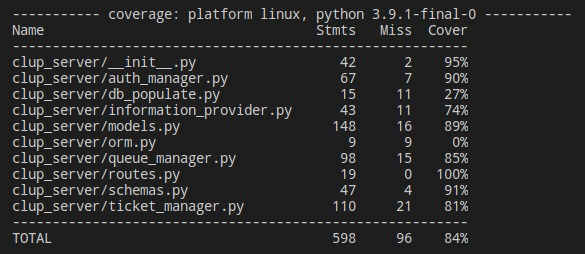
\includegraphics[width=\textwidth]{Images/coverage.jpeg}
    \caption{\label{fig:General Component}Statement Coverage}
\end{figure}